\documentclass[11pt]{article}

\usepackage[margin=1in]{geometry}
\usepackage{booktabs}
\usepackage{amsmath,amssymb}
\usepackage{url}
\usepackage[hidelinks]{hyperref}
\usepackage{listings}
\usepackage{xcolor}
\usepackage{pgfplots}
\usepackage{tikz}
\usetikzlibrary{positioning,fit,calc}

\pgfplotsset{compat=1.18}

\lstset{
  basicstyle=\ttfamily\footnotesize,
  breaklines=true,
  frame=single,
  backgroundcolor=\color{gray!8}
}

\title{Packing Logical KV Slices Under CUDA 2\,MiB Granularity:\\
42\% Measured VRAM Liberation on H100}

\author{
Stanislav Byriukov \\
Independent Researcher \\
\texttt{stanislav.byriukov.research@gmail.com}
}

\date{}

\begin{document}
\maketitle

\begin{abstract}
On NVIDIA H100 PCIe (driver 550.163), a user-space CUDA shim packing 512\,KiB logical KV bands into 2\,MiB driver leaves reduces \textbf{committed} VRAM by \textbf{42.2\%} at a 70\% VRAM budget fill while delivering \textbf{131\%} higher budget-curve logical KV than stock at the same tier (50\%/60\%: 19.1\%/32.6\% liberation).
The headline gain is a budget-curve ratio against growing stock commitment; matched-slot F1$'$ resident stress shows \textbf{0.15\%} slot gain and \textbf{100\%} vs \textbf{70.3\%} layout efficiency---the mechanism proof, not 131\%.

We intercept \texttt{cuMemAddressReserve}/\texttt{cuMemCreate}/\texttt{cuMemMap} via \texttt{lib2adic\_shim.so} and LD\_PRELOAD without application source changes.
Evaluation uses a \textbf{synthetic KV-band microbenchmark} with GATE12 transcripts and Docker reproduction: it isolates \emph{allocator/driver-layer} behavior from framework paging (vLLM PagedAttention operates above this layer).
\textbf{Track B} (production-stack vLLM integration) is a planned follow-up release, not part of tag \texttt{t1-eval-20260522}.
We do not claim inference P99, per-\texttt{cuMem*} alloc-path latency, FLOPS/W, or industry Z-scores in this paper.
\end{abstract}

\noindent\textbf{Keywords:} KV cache, CUDA, GPU memory, memory granularity, data structures, reproducible benchmark, GATE12.

\medskip
\noindent\textbf{Declaration on the use of AI language tools:}
Structure assisted by Cursor Agent; all benchmarks run on H100 by the author.
Generative tools did not execute GPU experiments and did not alter GATE12 metrics or reported tables.

\section{Introduction}

KV cache footprint dominates VRAM in long-context LLM inference~\cite{vllm,attention_is_all_you_need}.
Allocator behavior at the CUDA driver boundary---not only high-level frameworks---determines how many logical slots fit under a memory budget~\cite{cuda_prog_guide,cuda_driver_cuMem}.

\paragraph{Problem.}
When the platform enforces ${\sim}$2\,MiB minimum mapping granularity, mapping one 512\,KiB logical KV slice per leaf wastes physical commitment: only one quarter of the leaf carries application-visible KV bytes in the uniform-iso regime.
Frameworks may request sub-leaf logical regions; the stock path in our iron baseline still commits one 2\,MiB mapping per slot.

\paragraph{Approach.}
A shim intercepts \texttt{cuMem*} on the allocation path, reserves logical virtual spans, and packs multiple logical slots per 2\,MiB leaf (P1 policy, $k{\approx}4$ for 512\,KiB slices).
Mega-VA mode amortizes \texttt{cuMemAddressReserve} across resident pools used in multi-slot benches.

\paragraph{Contributions (measurement-backed only).}
\begin{enumerate}
  \item Iron-verified \texttt{leaf\_bytes=2097152} on H100 and P1 packing for uniform 512\,KiB iso slices.
  \item VRAM budget curve (50/60/70\% caps) with explicit stock-class pairing and plateau disclosure.
  \item Reproducible artifact: evaluation repository, Docker gate, fixed \texttt{workload\_id}, canonical GATE12 transcripts (Appendix~\ref{app:gate12}).
\end{enumerate}

\section{Background and Related Work}

\paragraph{CUDA virtual memory.}
Modern CUDA separates virtual address reservation from physical allocation~\cite{cuda_prog_guide,cuda_driver_cuMem}.
Our work operates at this boundary via LD\_PRELOAD---not kernel modules or eBPF.

\paragraph{LLM KV cache systems.}
Serving systems such as vLLM introduced paged KV attention to improve throughput~\cite{vllm}.
\textbf{We do not benchmark vLLM} in this paper; we cite them only as motivation for KV memory pressure.

\paragraph{GPU memory context.}
Accelerator memory pressure and pooling are surveyed in~\cite{sze2017efficient}.
Our shim is policy-specific to 2\,MiB CUDA leaves and measured KV-band workloads---not a general GPU allocator.

\paragraph{Author measurement line.}
Prior work~\cite{byriukov2026tal} documents iron GPU receipts (energy/latency) on H100-class hardware; it does \textbf{not} evaluate KV packing or CUDA \texttt{cuMem*} interception.

\section{Design}
\label{sec:design}

\subsection{Stock baseline}
For each logical slot the stock path issues \texttt{cuMemAddressReserve}, \texttt{cuMemCreate}, and \texttt{cuMemMap} with physical size 2\,MiB for requests up to 512\,KiB (iron \texttt{frag\_alloc\_bytes}).
Layout efficiency under uniform 512\,KiB logical bands is therefore at most $512\,\mathrm{KiB}/2\,\mathrm{MiB}=25\%$ before any framework overhead; F1$'$ resident measurement reports \textbf{70.3\%} on stock vs \textbf{100\%} on shim at matched stress (Table~\ref{tab:canonical}).

\subsection{Shim packing (P1 + mega)}
\begin{itemize}
  \item \textbf{P1 pack:} up to $k{=}4$ logical 512\,KiB slices share one \texttt{leaf\_bytes} leaf when placement rounds allow.
  \item \textbf{Mega-VA:} one large virtual reservation backs many resident slots; required for multi-slot pools without per-slot reserve storms.
  \item \textbf{Evaluation-only:} \texttt{lib2adic\_shim.so} + \texttt{iron\_gate\_v1}; production/unlimited binaries under separate license.
\end{itemize}

Figure~\ref{fig:packing} contrasts one 2\,MiB leaf under stock vs packed shim policy.

\begin{figure}[ht]
\centering
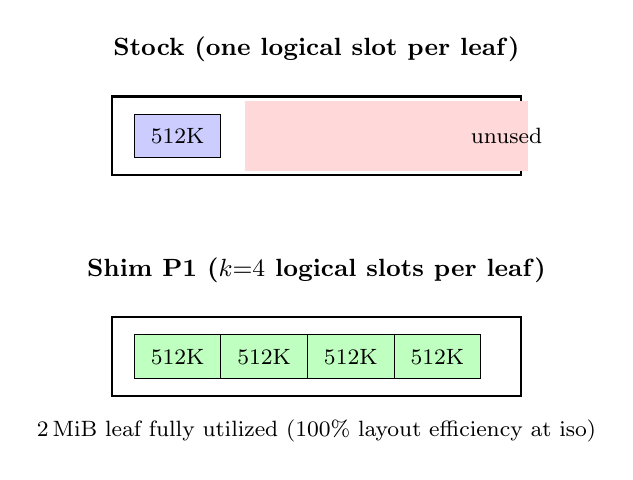
\begin{tikzpicture}[
  slot/.style={draw, minimum width=1.1cm, minimum height=0.55cm, font=\footnotesize},
  leaf/.style={draw, thick, inner sep=4pt},
  waste/.style={fill=red!15}
]
\node[font=\small\bfseries] at (0,2.3) {Stock (one logical slot per leaf)};
\node[leaf, minimum width=5.2cm, minimum height=1.0cm] (sleaf) at (0,1.2) {};
\node[slot, fill=blue!20] at ($(sleaf.west)+(0.85,0)$) {512K};
\node[waste, minimum width=3.6cm, minimum height=0.9cm, anchor=west] at ($(sleaf.west)+(1.7,0)$) {};
\node[font=\footnotesize] at ($(sleaf.east)+(-0.2,0)$) {unused};

\node[font=\small\bfseries] at (0,-0.5) {Shim P1 ($k{=}4$ logical slots per leaf)};
\node[leaf, minimum width=5.2cm, minimum height=1.0cm] (hleaf) at (0,-1.6) {};
\foreach \i/\x in {1/0.85, 2/1.95, 3/3.05, 4/4.15} {
  \node[slot, fill=green!25] at ($(hleaf.west)+(\x,0)$) {512K};
}
\node[font=\footnotesize, align=center] at (0,-2.55) {2\,MiB leaf fully utilized (100\% layout efficiency at iso)};
\end{tikzpicture}
\caption{Uniform 512\,KiB logical KV bands under 2\,MiB CUDA minimum leaf size.
Stock maps one band per leaf; shim packs four bands per leaf ($k{=}4$).}
\label{fig:packing}
\end{figure}

\subsection{Synthetic workloads}
All experiments use \texttt{workload\_id=a\_gate\_v1\_kv\_microbench}, \texttt{workload\_class=synthetic\_kv\_band}.
\begin{center}
\begin{tabular}{@{}llp{6.2cm}@{}}
\toprule
\texttt{stress\_mode} & Role & Notes \\
\midrule
\texttt{f1\_frag\_v1} & F1$'$ resident & Uniform 512\,KiB, 8\,s wall, separate stock/shim processes \\
\texttt{vram\_budget\_curve\_v1} & Budget curve & Iso fill to 50/60/70\% of GPU VRAM cap; \texttt{cache\_liberation\_method=iso\_logical\_v2} \\
\bottomrule
\end{tabular}
\end{center}

\section{Iron Measurement Protocol and GATE12}
\label{sec:iron}

\subsection{Hardware and run window}
All canonical numbers come from NVIDIA H100 PCIe, driver \textbf{550.163.01}, iron window 2026-05-22.
Each run emits JSON artifacts under \texttt{bench\_artifacts/} and a \texttt{GATE12\_BEGIN}...\texttt{GATE12\_END} stdout block for machine parsing.

\subsection{GATE12 contract}
GATE12 is the external metric surface: one line per field, no prose inside the block.
Required fields for curve runs include \texttt{leaf\_bytes}, per-tier \texttt{committed\_bytes\_*}, \texttt{resident\_slots\_*}, \texttt{cache\_liberation\_pct\_*}, and \texttt{logical\_kv\_gain\_pct\_*} (Appendix~\ref{app:curve}).
Partnership-facing summaries must copy from \texttt{results/GATE12\_canonical.txt} without hand rounding beyond 0.1\%.

\subsection{Metric definitions}
At matched budget tier $b$:
\begin{align*}
\texttt{cache\_liberation\_pct}_b &= \frac{C_{\mathrm{stock},b}-C_{\mathrm{shim},b}}{C_{\mathrm{stock},b}}\times 100, \\
\texttt{logical\_kv\_gain\_pct}_b &= \frac{L_{\mathrm{shim},b}-L_{\mathrm{stock},b}}{L_{\mathrm{stock},b}}\times 100, \\
\texttt{layout\_efficiency\_pct} &= \frac{L}{C}\times 100.
\end{align*}
\textbf{Stock-class pairing:} curve claims always name budget \% and report both committed totals; F1$'$ claims name \texttt{stress\_mode=f1\_frag\_v1} and 8\,s resident window.

\subsection{Comparison discipline}
\begin{itemize}
  \item Stock and shim runs are separate processes for resident/F1$'$ metrics (no cross-contamination).
  \item Shim env: \texttt{LD\_PRELOAD=lib2adic\_shim.so}, \texttt{HWATOM\_SHIM\_PACK=1}, \texttt{HWATOM\_PACK\_MEGA=1}.
  \item \textbf{Plateau check:} if \texttt{resident\_slots\_shim}=65536 while \texttt{committed\_shim} $<$ budget cap, liberation compares fair stock growth vs early shim ceiling---not ``shim fills entire budget.''
\end{itemize}

\subsection{Docker reproduction}
Image built from \texttt{docker/gate-12s/Dockerfile.f1prime}.
Success signal: \texttt{A46\_DOCKER\_OK} plus GATE12 fields matching bare-metal F1$'$ ordering (slot counts may differ in container cap).

\section{Results}
\label{sec:results}

\subsection{Measured leaf granularity}
VRAM curve GATE12 reports \texttt{leaf\_bytes=2097152} (2\,MiB) on H100 for the canonical run (\texttt{run\_id=1779431329}), anchoring the packing factor $k=4$ design for 512\,KiB iso slices.

\subsection{VRAM budget curve}
Table~\ref{tab:curve} lists all three budget tiers from \texttt{vram\_curve\_20260522T062629Z}.
Shim \texttt{committed\_bytes} plateaus at 34.36\,GiB (65536 slots $\times$ 512\,KiB logical layout policy) while stock committed grows with budget.

\begin{table}[ht]
\centering
\caption{VRAM budget curve (iso logical v2, H100, 2026-05-22).}
\label{tab:curve}
\small
\begin{tabular}{@{}cccccc@{}}
\toprule
Budget & $C_{\mathrm{stock}}$ (GiB) & $C_{\mathrm{shim}}$ (GiB) & Liberation & Log.\ gain & Slots (S / H) \\
\midrule
50\% & 39.55 & 32.00 & 19.1\% & +223\% & 20248 / 65536 \\
60\% & 47.46 & 32.00 & 32.6\% & +169\% & 24298 / 65536 \\
70\% & 55.36 & 32.00 & 42.2\% & +131\% & 28348 / 65536 \\
\bottomrule
\end{tabular}
\end{table}

\begin{figure}[ht]
\centering
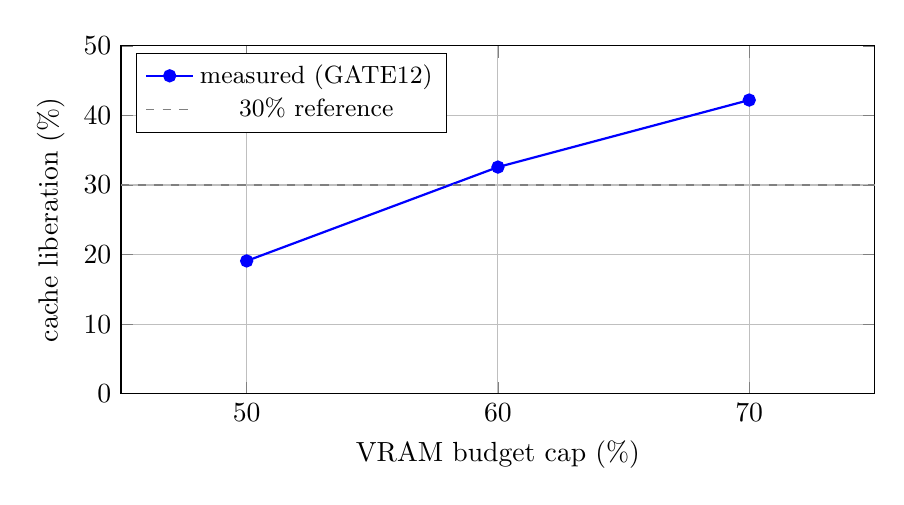
\begin{tikzpicture}
\begin{axis}[
  width=0.92\linewidth,
  height=6cm,
  ylabel={cache liberation (\%)},
  xlabel={VRAM budget cap (\%)},
  xmin=45, xmax=75,
  ymin=0, ymax=50,
  xtick={50,60,70},
  ytick={0,10,20,30,40,50},
  grid=major,
  legend style={at={(0.02,0.98)},anchor=north west,font=\small}
]
\addplot[mark=*,thick,blue] coordinates {(50,19.0834) (60,32.5706) (70,42.2040)};
\addlegendentry{measured (GATE12)}
\addplot[dashed,gray,domain=45:75,samples=2] {30};
\addlegendentry{30\% reference}
\end{axis}
\end{tikzpicture}
\caption{Cache liberation vs VRAM budget tier.
Liberation rises as stock committed scales; 50\% tier is below the 30\% audit band because stock has not yet scaled, not because packing failed.}
\label{fig:curve-lib}
\end{figure}

\begin{figure}[ht]
\centering
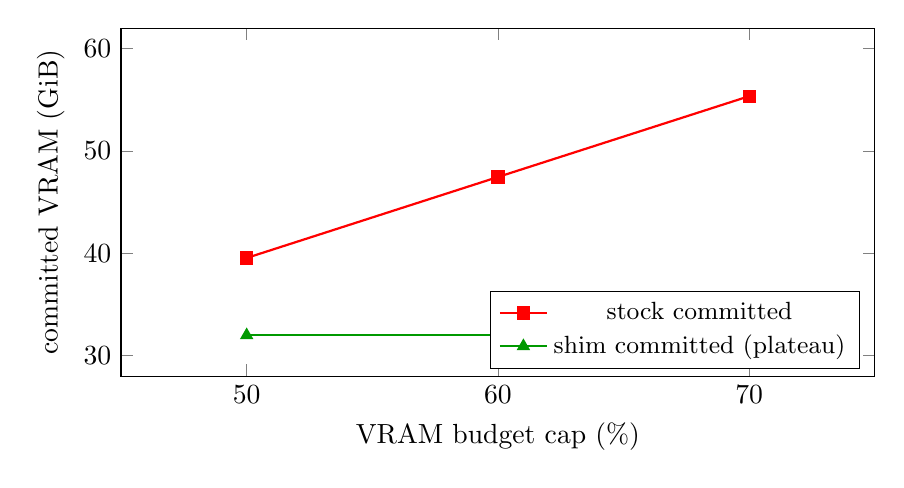
\begin{tikzpicture}
\begin{axis}[
  width=0.92\linewidth,
  height=6cm,
  ylabel={committed VRAM (GiB)},
  xlabel={VRAM budget cap (\%)},
  xmin=45, xmax=75,
  ymin=28, ymax=62,
  xtick={50,60,70},
  legend style={at={(0.98,0.02)},anchor=south east,font=\small}
]
\addplot[mark=square*,thick,red] coordinates {(50,39.55) (60,47.46) (70,55.36)};
\addlegendentry{stock committed}
\addplot[mark=triangle*,thick,green!60!black] coordinates {(50,32.00) (60,32.00) (70,32.00)};
\addlegendentry{shim committed (plateau)}
\end{axis}
\end{tikzpicture}
\caption{Committed bytes vs budget.
Shim hits slot/commit plateau before consuming the full 70\% budget cap.}
\label{fig:curve-commit}
\end{figure}

\subsection{F1$'$ resident uniformity}
Under \texttt{f1\_frag\_v1} with 8\,s resident window, stock holds 30{,}202 slots at 70.3\% layout efficiency; shim holds 30{,}248 slots at 100\% layout efficiency (\texttt{kv\_gain\_pct=0.15} at matched near-cap slot count).
This isolates packing geometry from budget-fill curve effects.

\subsection{Docker gate}
Container F1$'$ reproduces shim layout efficiency 100\% with \texttt{resident\_slots\_shim=29877} (stock 40{,}268 in same image cap), confirming the evaluation artifact path rather than bare-metal-only scripts.

\begin{table}[ht]
\centering
\caption{Canonical summary (2026-05-22, \texttt{results/GATE12\_canonical.txt}).
\textbf{131\%} is \texttt{logical\_kv\_gain\_pct} on the budget-fill curve (stock committed scales; shim plateaus).
F1$'$ row is matched-slot geometry (\texttt{kv\_gain\_pct}$\approx$0.15\%).}
\label{tab:canonical}
\begin{tabular}{@{}llrr@{}}
\toprule
Scenario & Metric & Stock & Shim \\
\midrule
VRAM @ 70\% & \texttt{cache\_liberation\_pct} & --- & \textbf{42.2\%} \\
VRAM @ 70\% & \texttt{logical\_kv\_gain\_pct} & --- & \textbf{+131\%} \\
VRAM @ 70\% & \texttt{committed\_bytes} & 59.45\,GB & 34.36\,GB \\
VRAM @ 70\% & \texttt{resident\_slots} & 28,348 & 65,536 \\
F1$'$ 8\,s & \texttt{resident\_slots} & 30,202 & 30,248 \\
F1$'$ 8\,s & \texttt{layout\_efficiency\_pct} & 70.3\% & \textbf{100\%} \\
Docker F1$'$ & \texttt{resident\_slots} & 40,268 & 29,877 \\
\bottomrule
\end{tabular}
\end{table}

\section{Discussion}

\paragraph{Why liberation grows along the curve.}
Packing factor $k$ is fixed for uniform 512\,KiB iso slices; liberation percentage is a \emph{ratio} against stock committed that increases as stock fills larger budget tiers while shim committed stays at the structural plateau.
Reporting only the 70\% point without 50/60\% misstates fair comparison protocol.

\paragraph{Mechanism ceiling (internal, not headline).}
A fixed 2\,GiB logical iso target can exhibit up to ${\sim}$75\% liberation ($k{=}4$ vs one band per 2\,MiB leaf).
Headline partnership numbers in this paper use the budget-fill curve unless explicitly labeled iso-fixed.

\paragraph{Relation to framework-level paging.}
vLLM's PagedAttention~\cite{vllm} manages logical KV pages above the CUDA driver via framework pool allocators, reducing per-slot \texttt{cuMem*} pressure on that code path.
Our shim is orthogonal at the driver API layer: it benefits stacks that still issue per-allocation \texttt{cuMem*} calls (custom PyTorch inference, some TRT-LLM pre-paging paths, and evaluation harnesses).
Integrating with vLLM's pool lifecycle is \textbf{Track B} (planned public integration release), not the T1 synthetic gate in Table~\ref{tab:canonical}.

\paragraph{Headline metrics vs mechanism.}
The \textbf{131\%} budget-curve logical KV gain is measured on the fill-to-budget curve where stock \texttt{committed\_bytes} grows and shim hits a structural plateau; it must not be read as ``131\% more KV per slot.''
F1$'$ at matched near-cap slots (\texttt{kv\_gain\_pct=0.15}) is the clean packing geometry readout.

\paragraph{Deployment economics.}
VRAM savings translate to concurrent capacity and cost only after integration on a customer serving stack; we do not state \$/GPU or utilization-dollar figures without production measurements.

\paragraph{What we defer.}
\textbf{Track B} vLLM end-to-end benchmarks, multi-GPU NCCL, GQA alias paths (iron-unstable), eBPF/kernel delivery (contract tier), and future \textbf{C-layer} SKU studies (e.g.\ B200-class iron) with fresh GATE12 runs.

\section{Limitations}
\begin{enumerate}
  \item Synthetic KV-band microbenchmark---isolates driver-layer packing; not transformer forward passes or Track B vLLM integration (planned separately).
  \item Single GPU SKU (H100 PCIe); \texttt{leaf\_bytes} may differ on other SKUs---re-measure before claiming portability (future C-layer/B200-class runs are out of scope here).
  \item Shim slot plateau (\texttt{ISO\_MAX\_SLOTS=65536}) at 34.36\,GiB committed under the 70\% budget scenario---a bench cap, not proof that shim consumes the full budget envelope.
  \item Per-call \texttt{cuMem*} allocation-path latency (stock vs shim) is \textbf{not} reported for T1 workloads in Table~\ref{tab:canonical}; separate scout tail benches (\texttt{kv\_tail\_latency\_v1}) exist in the evaluation repo annex but are excluded from this paper's claims.
  \item Docker slot caps differ from bare-metal F1$'$; compare layout efficiency and repro signals, not absolute slot parity across environments.
\end{enumerate}

\section{Reproducibility and Artifact}

Repository (URL at preview): \texttt{github.com/StanByriukov02/hwatom-gate-12s}, tag \texttt{t1-eval-20260522}~\cite{hardware_atom_t1}.

\begin{lstlisting}
git clone https://github.com/StanByriukov02/hwatom-gate-12s
cd hardware_atom
git checkout t1-eval-20260522
bash scripts/shim/run_docker_a46_gate12_f1prime_v1.sh
# Bare-metal iron (H100):
# bash scripts/shim/run_iron_vram_budget_curve_v1.sh
\end{lstlisting}

Expect \texttt{GATE12\_BEGIN}, \texttt{workload\_id=a\_gate\_v1\_kv\_microbench}, and tier fields matching Appendix~\ref{app:curve}.
Evaluation-Only \texttt{LICENSE.md}; production contact \texttt{stanislav.byriukov.research@gmail.com}.

\paragraph{Frozen table policy.}
Public eval Docker may add \texttt{HWATOM\_PACK\_K\_CAP} after tag \texttt{t1-eval-20260522}; Tables~\ref{tab:curve}--\ref{tab:canonical} remain tied to iron/H100 measurements at that tag.

\appendix

\section{Full GATE12 transcripts}
\label{app:gate12}

\subsection{VRAM budget curve}
\label{app:curve}
\begin{lstlisting}
GATE12_BEGIN
workload_id=a_gate_v1_kv_microbench
workload_class=synthetic_kv_band
stress_mode=vram_budget_curve_v1
cache_liberation_method=iso_logical_v2
leaf_bytes=2097152
gpu_sku=NVIDIA H100 PCIe
driver_version=550.163.01
vram_budget_pct_50=50
cache_liberation_pct_50=19.0834
logical_kv_gain_pct_50=223
committed_bytes_stock_50=42463133696
committed_bytes_shim_50=34359738368
vram_budget_pct_60=60
cache_liberation_pct_60=32.5706
logical_kv_gain_pct_60=169
vram_budget_pct_70=70
cache_liberation_pct_70=42.2040
committed_bytes_stock_70=59450064896
committed_bytes_shim_70=34359738368
resident_slots_stock_70=28348
resident_slots_shim_70=65536
logical_kv_gain_pct_70=131
GATE12_END
\end{lstlisting}
\emph{Source:} \texttt{bench\_artifacts/h100\_pull\_20260522/vram\_curve\_20260522T062629Z/}.

\subsection{F1$'$ resident}
\begin{lstlisting}
GATE12_BEGIN
stress_mode=f1_frag_v1
resident_slots_stock=30202
resident_slots_shim=30248
layout_efficiency_stock=70.3136
layout_efficiency_shim=100.0000
kv_gain_pct=0.1523
elapsed_s=8.000
GATE12_END
\end{lstlisting}
\emph{Source:} \texttt{gate12\_f1prime\_20260522T064350Z/}.

\section{Claim checklist (submit)}
\begin{itemize}
  \item Abstract states \textbf{synthetic} workload and denies inference/Z claims.
  \item Primary arXiv category: \textbf{cs.DS}; optional cross-list cs.DC / cs.LG.
  \item Numbers match \texttt{GATE12\_canonical.txt} and Appendix~\ref{app:curve}.
  \item Git tag \texttt{t1-eval-20260522} live before upload (replace [TBD] URL).
\end{itemize}

\bibliographystyle{plain}
\bibliography{references}

\end{document}
